\section{Experiments}
\label{sec:experiments}
\subsection{Setup}
We evaluate 770 queries from five query sets---TREC-DL 2019/2020, NFCorpus, SciFact, and TREC-COVID---and the same 30 queries across five TREC-COVID snapshots~\cite{dl19,dl20,nfcorpus,scifact,covid}. We replay exact rankings from bge-small-en-v1.5~\cite{bge} and BM25~\cite{bm25} ($k_1=0.9$, $b=0.4$), using equal-weight RRF with contributions $1/(59+r)$ and deterministic tie breaking.

First, we choose $L$ on calibration queries and test it on held-out queries and later corpus snapshots. Next, we measure how many accesses are needed to complete exact Top-$k$ and when each result becomes certain. We then compare DiBud with Balanced under the same budgets and certification rules. Balanced alternates between the two lists. Budgets range from 128 to 10000, and we count certified results up to 20 and 100. Both methods access one entry at a time; we also test batches of 64.

Finally, we compare budgeted stopping with completing exact Top-20. Budgets are selected on calibration queries to retain 90\%, 95\%, or 99\% of the reference mean nDCG@20. We report the quality retained and accesses saved on held-out queries.

Results are averaged within each query set, then equally across sets. Where reported, 95\% confidence intervals use 2000 query bootstrap samples. Queries that reach the end of the saved rankings remain in the analysis, with bounds reported for outcomes that cannot be determined.

\subsection{Transfer of fixed depths}
Depths are 10, 20, 50, 100, 200, 500, 1000, 2000, and 5000. Five-fold calibration selects the depth with the highest mean linear-gain nDCG@10 on four folds, breaking ties toward smaller depths, and evaluates it on the held-out fold. Temporal calibration uses only Round-1 calibration topics and freezes the selection for disjoint held-out topics across all rounds. Bootstrap intervals reselect depths within calibration samples.
\begin{table}[t]
\centering
\caption{Five-fold query transfer of the depth selected by calibration nDCG@10. Agreement is exact ordered Top-20 agreement with full-list RRF, distinct from relevance quality.}
\label{tab:transfer}
\small
\setlength{\tabcolsep}{3pt}
\begin{tabular}{lrrr}
\toprule
Query set & Frozen $L$ & Full RRF & Agreement (\%) \\
\midrule
TREC-DL 2019 & 0.6798 & 0.6812 & 90.7 \\
TREC-DL 2020 & 0.6424 & 0.6243 & 0.0 \\
NFCorpus & 0.3665 & 0.3665 & 98.5 \\
SciFact & 0.7437 & 0.7442 & 32.3 \\
TREC-COVID & 0.8031 & 0.8059 & 44.0 \\
\bottomrule
\end{tabular}
\end{table}

Similar relevance scores do not imply similar fused rankings (Table~\ref{tab:transfer}). On SciFact, the selected depths attain nDCG@10 of 0.7437 versus 0.7442 for full-list RRF, but exact ordered Top-20 agreement is only 32.33\%. On TREC-DL 2020, the selected $L=20$ has higher held-out nDCG@10 (0.6424 versus 0.6243), while ordered agreement is zero. Truncation can be effective for relevance without reproducing full-list fusion.
\begin{figure}[tbp]
\centering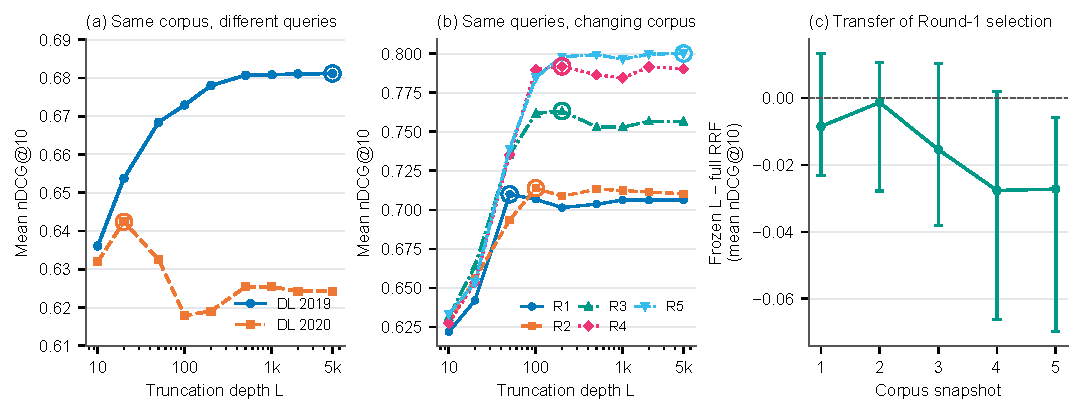
\includegraphics[width=\columnwidth]{../../../figures/paper-v2/transfer.pdf}
\caption{Fixed-depth transfer. Differences compare the frozen calibration selection with full-list RRF on the same held-out queries. Intervals are nested bootstrap 95\% intervals with depth reselection; temporal resampling preserves query identities across snapshots.}
\label{fig:transfer}\end{figure}
Across snapshots, the five fold-specific depths are 50, 50, 100, 1000, and 50, giving 500 mean accesses. The nDCG@10 difference from full-list RRF changes from $-0.0085$ in Round 1 to $-0.0272$ in Round 5; the latter has a paired 95\% interval of $[-0.0699,-0.0058]$. The change is not monotonic (Fig.~\ref{fig:transfer}). The frozen choice does not maintain the same relative effectiveness in this sequence. Comparisons remain within snapshot because judgments also change.

\subsection{Fixed-K cost and incremental certification}
\begin{table}[t]
\centering
\caption{Sorted accesses to exact Top-20 under unit SNRA. Completion is observed within the saved rankings and 10,000-access limit; unresolved P95 values are lower bounds.}
\label{tab:cost}
\small
\setlength{\tabcolsep}{3pt}
\begin{tabular}{lrrrr}
\toprule
Query set & $n$ & Median & P95 & Complete (\%) \\
\midrule
TREC-DL 2019 & 43 & 311 & $\geq 9108$ & 81.4 \\
TREC-DL 2020 & 54 & 444 & $\geq 9912$ & 85.2 \\
NFCorpus & 323 & 308 & 2685 & 100.0 \\
SciFact & 300 & 325 & 3362 & 100.0 \\
TREC-COVID & 50 & 2544 & $\geq 9842$ & 66.0 \\
\bottomrule
\end{tabular}
\end{table}

For exact Top-20, median access counts range from 308 to 2544 (Table~\ref{tab:cost}). All NFCorpus and SciFact queries complete within the observed range, but their P95 costs are 2685 and 3362, respectively: 8.72 and 10.34 times their medians. On the two TREC-DL sets and TREC-COVID, 18.60\%, 14.81\%, and 34.00\% of queries do not complete within the observed range. Their costs cannot be replaced by statistics over completed queries.
\begin{figure}[tbp]
\centering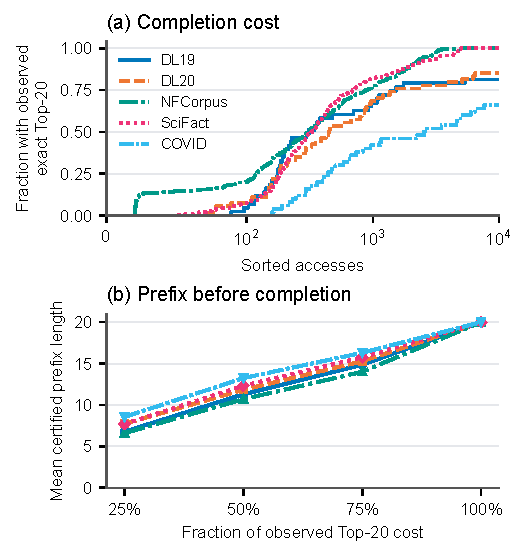
\includegraphics[width=\columnwidth]{../../../figures/paper-v2/cost.pdf}
\caption{Exact Top-20 completion and earlier certified output. (a) Observed completions divided by all queries; plateaus retain unresolved queries in the denominator. (b) Output at fractions of each query's observed completion cost, conditional on completion. This retrospective normalization is not an online policy.}
\label{fig:cost}\end{figure}
Among queries with observed Top-20 completion, half of the eventual accesses already certify 11.87 results on an equal-set average. The largest single certification increment accounts for 25.42\% of total accesses on average. Thus, useful prefixes are available before the fixed-size result is complete, although the measurements do not imply that every query is dominated by one extreme position (Fig.~\ref{fig:cost}).

\subsection{Certified output under equal budgets}
\begin{table}[t]
\centering
\caption{Mean certified output at $B=2048$. Both methods use unit accesses and the same certifier; only list selection differs.}
\label{tab:yield}
\small
\setlength{\tabcolsep}{3pt}
\begin{tabular}{lrrrr}
\toprule
& \multicolumn{2}{c}{Cap 100} & \multicolumn{2}{c}{Cap 20} \\ Query set & Balanced & DiBud & Balanced & DiBud \\
\midrule
TREC-DL 2019 & 41.86 & 46.19 & 17.77 & 17.91 \\
TREC-DL 2020 & 34.91 & 38.31 & 18.33 & 18.35 \\
NFCorpus & 62.06 & 63.71 & 19.24 & 19.28 \\
SciFact & 43.55 & 47.26 & 19.44 & 19.57 \\
TREC-COVID & 26.48 & 29.80 & 15.58 & 15.78 \\
\bottomrule
\end{tabular}
\end{table}

At $B=2048$, DiBud increases mean certified output within the first 100 positions from 41.77 to 45.05, a 7.86\% gain over Balanced (Table~\ref{tab:yield}). Within the first 20 positions, the mean changes from 18.07 to 18.18. All five sets gain output, with larger improvements for longer prefixes. The macro fraction returning at least 20 results increases from 75.10\% to 76.22\%; average prefix growth and complete-20 delivery are distinct outcomes.
\begin{figure*}[t]
\centering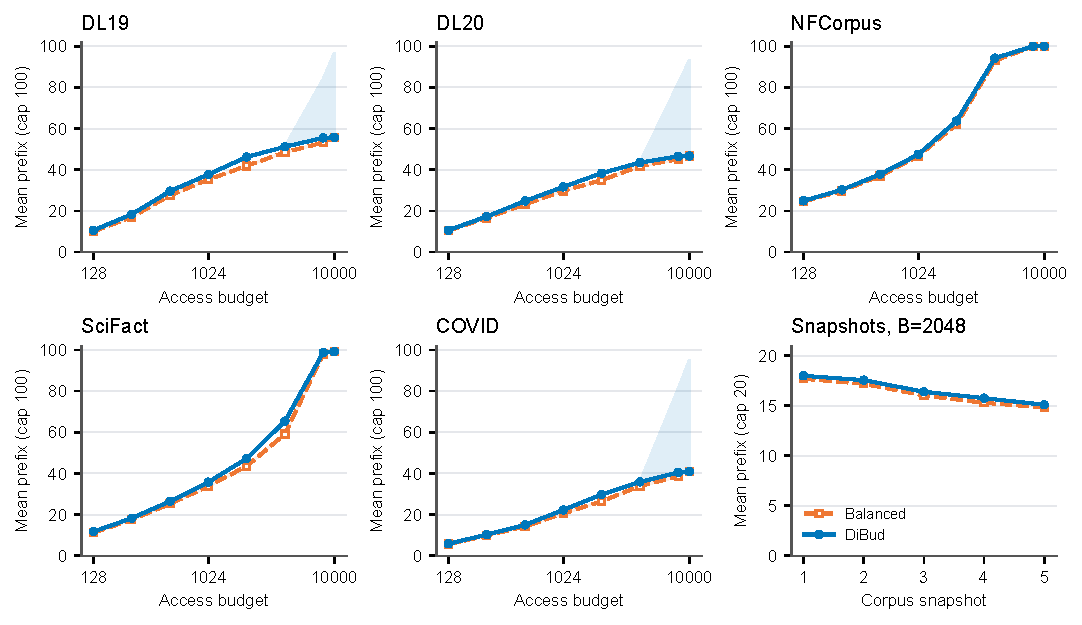
\includegraphics[width=\textwidth]{../../../figures/paper-v2/yield.pdf}
\caption{Certified output versus budget and snapshot. Shading bounds output after a saved-list observation limit; it is not a confidence interval. Static panels use a reporting cap of 100. The snapshot panel uses cap 20 and $B=2048$, where all endpoints are observed.}
\label{fig:yield}\end{figure*}
Over the full log-budget range, the lower bound on DiBud's normalized certified-prefix area exceeds Balanced's upper bound on every static set. Some asymmetric paths reach the saved-list limit at large budgets, so Fig.~\ref{fig:yield} shows intervals rather than treating the retained prefix as the final output. The lower bound on the area difference remains positive when both schedules use batches of 64. The gain is therefore not solely a unit-access effect.

Across the five snapshots at $B=2048$, DiBud returns means of 18.00, 17.57, 16.40, 15.77, and 15.10 results within the first 20 positions, versus 17.70, 17.20, 16.03, 15.30, and 14.83 for Balanced. A fixed budget yields different output sizes as the corpus changes. DiBud improves the mean in every round. Full budget curves, output quantiles, empty-output rates, and delivery thresholds are retained with the experiment artifacts.

\subsection{Quality and access cost relative to exact Top-20}
We compare two stopping conditions on the same unit-SNRA trajectory: complete exact Top-20, or stop at the budget or at 20 certified results, whichever comes first. Evaluation uses linear-gain nDCG@20, with absent positions contributing zero. For each query set, five-fold calibration chooses the smallest budget retaining 90\%, 95\%, or 99\% of the reference mean nDCG@20; the frozen choice is evaluated on held-out queries. Retention is a ratio of means, not a mean of per-query ratios with an arbitrary value for zero-reference queries.
\begin{table}[t]
\centering
\caption{Held-out Top-20 comparison after selecting the smallest budget retaining 95\% of reference mean nDCG@20 on calibration queries. Retention is a ratio of dataset means. Intervals and $\geq$ reflect unobserved continuations, not confidence intervals.}
\label{tab:quality}
\small
\setlength{\tabcolsep}{3pt}
\begin{tabular}{lrrr}
\toprule
Query set & Retained (\%) & Fewer accesses (\%) & Top20 (\%) \\
\midrule
TREC-DL 2019 & 95.05 & $\geq 76.02$ & 67.4 \\
TREC-DL 2020 & 95.89 & $\geq 70.96$ & 68.5 \\
NFCorpus & 95.81 & 65.92 & 52.3 \\
SciFact & 97.68 & 83.41 & 11.3 \\
TREC-COVID & 95.14--96.43 & $\geq 5.30$ & 64.0 \\
\bottomrule
\end{tabular}
\end{table}

At the 95\% calibration target, NFCorpus and SciFact retain 95.81\% and 97.68\% of held-out nDCG@20 while reducing accesses by 65.92\% and 83.41\% (Table~\ref{tab:quality}). TREC-DL 2019/2020 retain 95.05\% and 95.89\%. Their all-query access reductions are at least 76.02\% and 70.96\%, using lower bounds on unresolved exact Top-20 costs. Within the completed-query subsets alone, reductions are 35.70\% and 47.07\%, illustrating the influence of difficult queries on total cost.
\begin{figure}[tbp]
\centering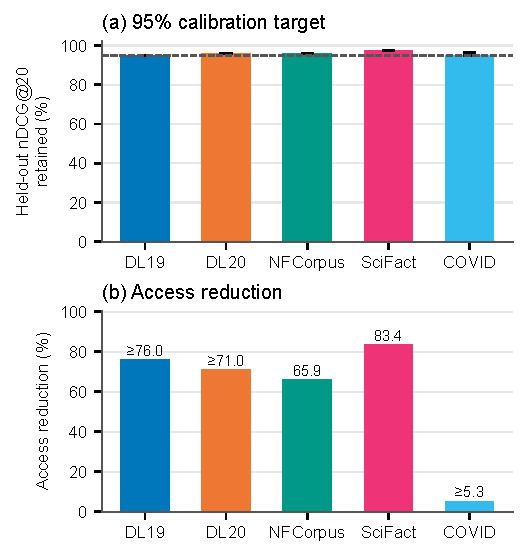
\includegraphics[width=\columnwidth]{../../../figures/paper-v2/quality-cost.pdf}
\caption{Held-out quality and access reduction relative to exact Top-20 after 95\% calibration. The dashed line is the calibration target, not a per-query guarantee. A range denotes unobserved continuation; reduction labels with $\geq$ are conservative bounds.}
\label{fig:quality}\end{figure}
TREC-COVID requires a different tradeoff: retention is bounded by 95.14\%--96.43\%, while access reduction is guaranteed only to be at least 5.30\%. At the 99\% target, five, four, and five calibration folds on TREC-DL 2019, TREC-DL 2020, and TREC-COVID fail to establish the target from the available rankings. These are not successful target crossings.

Budgeted stopping can therefore retain much of the top-ranked relevance gain while reducing accesses spent completing Top-20, at the cost of output size. At the 95\% target, only 52.32\% of NFCorpus queries and 11.33\% of SciFact queries return all 20 results. Quality retention is not a substitute for result coverage or a guarantee for each query.
